\chapter{Lichtkegel, Geodäten und der Schwarzschild-Horizont}

Das Horizontproblem beginnt mit einer Unterscheidung, die bereits in der speziellen Relativitätstheorie auftritt. Zwei benachbarte Ereignisse können zeitartig, raumartig oder lichtartig voneinander getrennt sein. Die Krümmung hebt diese Klassifikation nicht auf. Sie macht den Lichtkegel zu einem lokalen Objekt, das an jedem Ereignis anders ist, und lässt die Metrik selbst dynamisch werden. Ist die Metrik bekannt, folgt die Bewegung eines frei fallenden Teilchens aus demselben Eigenzeitprinzip, das ein freies relativistisches Teilchen in der flachen Raumzeit beschreibt.

Wir werden dieses Prinzip zweimal anwenden. Zunächst muss es die Newtonsche Bewegung in einem schwachen Feld wiedergeben. Anschließend wenden wir es auf die Schwarzschild-Metrik an, in der sich die Bedeutung von Zeit, radialem Abstand und Geschwindigkeit als unerwartet subtil erweist.

\section{Zeitartige, raumartige und lichtartige Intervalle}

In der flachen Raumzeit mit \(c=1\) lautet das Eigenzeitelement
\begin{equation}
d\tau^2=dt^2-dx^2-dy^2-dz^2.
\label{eq:l5-minkowski-proper-time}
\end{equation}
Die Rückkehr zu \(c\) ist hilfreich, wenn eine nichtrelativistische Näherung naheliegt:
\begin{equation}
d\tau^2
=dt^2-\frac{dx^2+dy^2+dz^2}{c^2}.
\label{eq:l5-minkowski-c}
\end{equation}
Die Schreibweise \(d\tau^2\) garantiert nicht, dass die rechte Seite positiv ist. Ihr Vorzeichen klassifiziert die Verschiebung:
\begin{align}
d\tau^2>0
&\quad\Longleftrightarrow\quad \text{time-like},\\
d\tau^2=0
&\quad\Longleftrightarrow\quad \text{light-like},\\
d\tau^2<0
&\quad\Longleftrightarrow\quad \text{space-like}.
\end{align}
Für eine raumartige Verschiebung ist es zweckmäßig, den positiven Eigenabstand zu definieren:
\begin{equation}
ds^2=-d\tau^2
=dx^2+dy^2+dz^2-dt^2
\qquad(c=1).
\label{eq:l5-proper-distance}
\end{equation}

Der Lichtkegel ordnet diese drei Möglichkeiten. Seine Oberfläche, nicht sein ausgefüllter Innenbereich, besteht aus den lichtartigen Richtungen. Zeitartige Richtungen liegen innerhalb des Kegels, raumartige außerhalb. Die obere und die untere Hälfte stellen den zukünftigen beziehungsweise den vergangenen Lichtkegel dar.

\begin{figure}[htbp]
\centering
\includegraphics[width=0.82\textwidth]{lecture_05_figure_02.png}
\caption{Eigenzeit, Eigenabstand und der Kausalkegel, wie sie an der Tafel zusammengestellt wurden. Lichtstrahlen liegen auf dem Kegel selbst; sein Inneres ist zeitartig, sein Äußeres raumartig.}
\lectureframe{00:05:44}
\end{figure}

\begin{figure}[htbp]
\centering
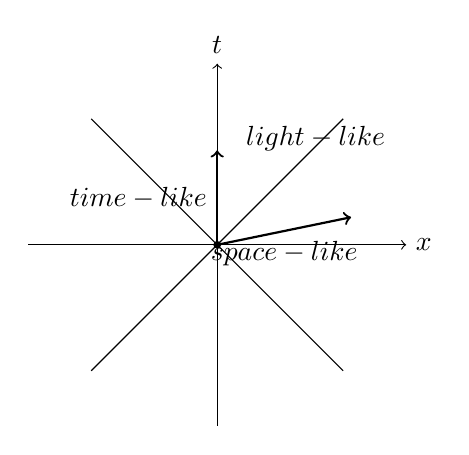
\begin{tikzpicture}[scale=1.0]
\draw[->] (0,-2.3) -- (0,2.3) node[above] {\(t\)};
\draw[->] (-2.4,0) -- (2.4,0) node[right] {\(x\)};
\draw (-1.6,1.6) -- (0,0) -- (1.6,1.6);
\draw (-1.6,-1.6) -- (0,0) -- (1.6,-1.6);
\fill (0,0) circle (1.4pt);
\draw[->,thick] (0,0) -- (0,1.2)
  node[midway,left] {\(\text{time-like}\)};
\draw[->,thick] (0,0) -- (1.7,0.35)
  node[midway,below] {\(\text{space-like}\)};
\node at (1.25,1.35) {\(\text{light-like}\)};
\end{tikzpicture}
\caption{Die kausale Klassifikation in einem zweidimensionalen Raumzeitabschnitt.}
\end{figure}

Diese Intervalle haben eine operationale Bedeutung. Die Eigenzeit ist die Zeit, die eine Uhr entlang einer zeitartigen Weltlinie anzeigt. Den Eigenabstand zwischen raumartig getrennten Ereignissen misst ein geeigneter Satz von Maßstäben. Es handelt sich nicht bloß um Bezeichnungen für Vorzeichen in einer quadratischen Form.

\section{Lorentzsche Signatur und ein Kegel an jedem Ereignis}

In der Konvention mit überwiegend positiven Vorzeichen hat die flache Metrik die Komponenten
\begin{equation}
\eta_{\mu\nu}=\operatorname{diag}(-1,1,1,1),
\label{eq:l5-eta}
\end{equation}
und
\begin{equation}
d\tau^2=-\eta_{\mu\nu}\,dx^\mu dx^\nu.
\label{eq:l5-proper-time-eta}
\end{equation}
Die dargestellte Matrix ist die Darstellung eines Tensors zweiten Ranges in einer besonders einfachen Basis. Ihre invariante Eigenschaft ist ihre Signatur: eine negative und drei positive Richtungen,
\begin{equation}
\operatorname{signature}(\eta)=(-,+,+,+).
\label{eq:l5-lorentz-signature}
\end{equation}
Eine Metrik mit zwei negativen Vorzeichen hätte zwei zeitartige Richtungen. Solche Signaturen lassen sich mathematisch untersuchen, beschreiben aber nicht die hier vorausgesetzte Raumzeit.

In einer gekrümmten Raumzeit variieren die Komponenten:
\begin{equation}
g_{\mu\nu}=g_{\mu\nu}(x).
\label{eq:l5-position-metric}
\end{equation}
An jedem Ereignis muss die Metrik weiterhin Lorentzsche Signatur haben. Daher besitzt jedes Ereignis seine eigenen zeitartigen Richtungen, lichtartige Grenzrichtungen und raumartigen Richtungen. In einer Koordinatendarstellung können die Kegel von Punkt zu Punkt geneigt oder gestaucht erscheinen; die kausale Klassifikation bleibt jedoch erhalten.

\begin{figure}[htbp]
\centering
\includegraphics[width=0.86\textwidth]{lecture_05_figure_03.png}
\caption{Die ortsabhängige Metrik \(g_{\mu\nu}(x)\), die kausalen Bezeichnungen und Skizzen lokaler Lichtkegel.}
\lectureframe{00:09:41}
\end{figure}

\begin{figure}[htbp]
\centering
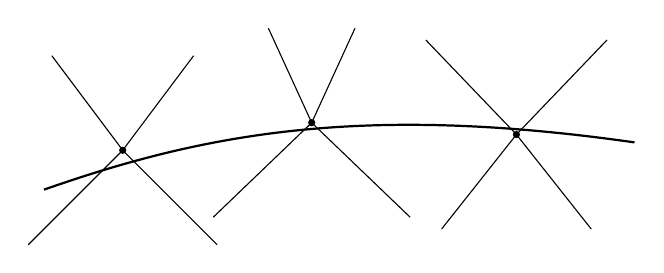
\begin{tikzpicture}[scale=1.0]
\draw[thick] (-4,-0.5) .. controls (-2,0.2) and (0,0.6) .. (3.5,0.1);
\foreach \x/\y/\a/\b in {-3/0/0.9/1.2, -0.6/0.35/0.55/1.25,
                          2.0/0.2/1.15/0.95} {
  \fill (\x,\y) circle (1.3pt);
  \draw (\x,\y) -- ++(-\a,1.2);
  \draw (\x,\y) -- ++(\a,1.2);
  \draw (\x,\y) -- ++(-\b,-1.2);
  \draw (\x,\y) -- ++(\b,-1.2);
}
\end{tikzpicture}
\caption{Benachbarte lokale Kegel. Ihre Koordinatenform kann sich ändern, ohne dass sich ändert, welche Vektoren zeitartig, lichtartig oder raumartig sind.}
\end{figure}

\begin{classroomqa}
\audiencequestion{Wählt der einzelne negative Eigenwert eine eindeutige Zeitrichtung aus?}
\lecturerresponse{Eine Basis, in der die dargestellte Matrix diagonal ist, hat eine negative Basisrichtung. Das wählt jedoch weder einen bevorzugten Beobachter noch eine eindeutige physikalische Zeitrichtung aus. Lorentz-Transformationen mischen die Zeitkoordinate mit den Raumkoordinaten, und jeder Vektor im Inneren des Kegels ist zeitartig. Das invariante Objekt ist der Kegel zusammen mit der Signatur mit einem Minus und drei Pluszeichen, nicht ein einzelner ausgezeichneter zeitartiger Vektor.
\lecturetimestamp{00:12:17--00:17:24}}
\end{classroomqa}

\begin{classroomqa}
\audiencequestion{Warum können zwei Zeichnungen des lokalen Kegels unterschiedlich aussehen?}
\lecturerresponse{Koordinaten können die Zeichnung verändern. Ersetzt man zum Beispiel \(x\) durch eine skalierte Koordinate, ändert sich die numerische Steigung, die einem Lichtstrahl zugeordnet wird; dadurch erscheint der Kegel schmaler oder breiter. Allgemeinere Koordinaten können ihn neigen. Dargestellt werden dabei dasselbe Ereignis und dieselben kausalen Beziehungen. In einer gekrümmten Raumzeit gehören Kegel an verschiedenen Ereignissen außerdem zu verschiedenen Tangentialräumen; für ihren Vergleich benötigt man daher die Metrik und eine Transportvorschrift.
\lecturetimestamp{00:13:37--00:15:59}}
\end{classroomqa}

\section{Geodäten als Variationsproblem}

Ein frei bewegliches Teilchen folgt einer Raumzeitgeodäte. In Differentialform lautet die Gleichung für einen affinen Parameter \(\lambda\):
\begin{equation}
\frac{d^2x^\mu}{d\lambda^2}
+\Gamma^\mu{}_{\rho\sigma}
\frac{dx^\rho}{d\lambda}
\frac{dx^\sigma}{d\lambda}=0.
\label{eq:l5-geodesic}
\end{equation}
Die Verbindung gibt an, wie der Tangentialvektor parallel zu sich selbst bleibt, während sich das Teilchen bewegt.

Es gibt eine zweite Formulierung, mit der sich oft leichter rechnen lässt. In einem Riemannschen Raum mit Metrik \(g_{mn}\) beträgt die Länge einer Kurve
\begin{equation}
s=\int ds
=\int\sqrt{g_{mn}\,dx^m dx^n}.
\label{eq:l5-spatial-length}
\end{equation}
Die Geodäte macht diese Länge bei kleinen Variationen des Weges mit festen Endpunkten stationär. Das Integral ist schlicht die Summe der infinitesimalen Längen entlang der Kurve, und die Euler--Lagrange-Gleichung ist eine Differentialgleichung zweiter Ordnung, die in ihrer Form einem Kraftgesetz ähnelt.

Bei einer zeitartigen Weltlinie tritt an die Stelle der räumlichen Länge die Eigenzeit:
\begin{equation}
\tau
=\int\sqrt{-g_{\mu\nu}\,dx^\mu dx^\nu}.
\label{eq:l5-proper-time-functional}
\end{equation}
Eine zeitartige Geodäte macht \(\tau\) stationär und ist für benachbarte frei fallende Wege lokal maximal, solange noch keine konjugierten Punkte auftreten. Multiplikation mit \(-m\) ergibt die Teilchenwirkung
\begin{equation}
A=-m\tau
=-m\int\sqrt{-g_{\mu\nu}\,dx^\mu dx^\nu}.
\label{eq:l5-particle-action}
\end{equation}
Derselbe Weg minimiert also lokal \(A=-m\tau\). Die Unterscheidung zwischen einer stationären Eigenzeit und dem Vorzeichen der gewählten Wirkung beseitigt den scheinbaren Widerspruch zwischen Minimum und Maximum.

\section{Von der Eigenzeit zur gewöhnlichen Lagrange-Funktion}

Die Wirkung in \eqref{eq:l5-particle-action} ist geometrisch, lässt sich aber in die aus der Mechanik vertraute Form bringen. Parametrisiert man die Weltlinie durch die Koordinate \(t\), dividiert jedes Differential durch \(dt\) und zieht den verbleibenden Faktor \(dt\) vor die Wurzel, erhält man:
\begin{align}
A
&=-m\int\sqrt{-g_{\mu\nu}(x)\,dx^\mu dx^\nu}\\
&=-m\int
\sqrt{-g_{\mu\nu}(x)
\frac{dx^\mu}{dt}\frac{dx^\nu}{dt}}\,dt.
\label{eq:l5-action-t}
\end{align}
Für die Zeitkomponente gilt \(dt/dt=1\); die Raumkomponenten sind gewöhnliche Koordinatengeschwindigkeiten. Daher können wir schreiben:
\begin{equation}
\begin{aligned}
A&=\int L\,dt,\\
L&=-m\sqrt{-g_{\mu\nu}(x)\dot x^\mu\dot x^\nu},\\
\dot x^\mu&=\frac{dx^\mu}{dt}.
\end{aligned}
\label{eq:l5-relativistic-lagrangian}
\end{equation}

\begin{figure}[htbp]
\centering
\includegraphics[width=0.88\textwidth]{lecture_05_figure_05.png}
\caption{Die Weltlinienwirkung wird in die übliche Form \(A=\int L\,dt\) überführt.}
\lectureframe{00:27:00}
\end{figure}

\begin{figure}[htbp]
\centering
\includegraphics[width=0.88\textwidth]{lecture_05_figure_06.png}
\caption{Ein späterer Tafelstand, auf dem die relativistische Lagrange-Funktion herausgearbeitet ist.}
\lectureframe{00:28:59}
\end{figure}

\begin{classroomqa}
\audiencequestion{Sollten die Raumzeitindizes in dieser Wirkung griechisch sein?}
\lecturerresponse{Ja. Griechische Indizes laufen über die Zeit- und alle Raumkoordinaten. Lateinische Indizes können den Raumkoordinaten vorbehalten bleiben, wenn diese Unterscheidung nützlich ist.
\lecturetimestamp{00:25:53--00:26:03}}
\end{classroomqa}

\begin{classroomqa}
\audiencequestion{Warum nennt man den Ausdruck unter der Wurzel die Lagrange-Funktion?}
\lecturerresponse{Sobald die Wirkung als \(A=\int L\,dt\) geschrieben ist, ist der Integrand die Lagrange-Funktion. Das ist nicht bloß eine Definition: Die Variation dieses Integranden ergibt die Euler--Lagrange-Gleichungen
\[
\frac{d}{dt}
\left(\frac{\partial L}{\partial\dot x^\mu}\right)
=\frac{\partial L}{\partial x^\mu},
\]
die bei konsistenter Behandlung der Parametrisierung äquivalent zur Geodätengleichung sind.
\lecturetimestamp{00:28:36--00:29:02}}
\end{classroomqa}

Für ein massives Teilchen ist die Weltlinie zeitartig, daher ist der Ausdruck unter der Wurzel positiv. Ein raumartiger Weg würde überlichtschnelle Bewegung beschreiben, nicht die Bahn eines gewöhnlichen massiven Teilchens. Ist die Metrik gegeben, lässt sich die Bahn des Teilchens entweder durch Berechnung der Christoffelsymbole und Anwendung von \eqref{eq:l5-geodesic} oder durch Anwendung der Euler--Lagrange-Gleichung auf \eqref{eq:l5-relativistic-lagrangian} bestimmen. Ihre Äquivalenz zu zeigen, ist eine nützliche Übung; der Weg über die Wirkung ist in der Regel kürzer.

\section{Der Newtonsche Grenzfall}

Betrachten wir das schwache, statische Gravitationsfeld außerhalb einer kugelförmigen Quelle. Wir beginnen mit der flachen Raumzeit und lassen den Koeffizienten von \(dt^2\) geringfügig von eins abweichen:
\begin{equation}
d\tau^2
=\left(1+\frac{2u(\mathbf{x})}{c^2}\right)dt^2
-\frac{d\mathbf{x}^2}{c^2},
\label{eq:l5-weak-metric}
\end{equation}
wobei \(u\) das Newtonsche Potential werden soll. Dieser Ansatz muss überprüft und darf nicht bloß so bezeichnet werden.

Die Teilchenwirkung mit ihren physikalischen Dimensionen lautet
\begin{equation}
A=-mc^2\int
\sqrt{1+\frac{2u}{c^2}
-\frac{\dot{\mathbf{x}}^{\,2}}{c^2}}\,dt.
\label{eq:l5-weak-action}
\end{equation}
Sowohl \(u/c^2\) als auch \(\dot{\mathbf{x}}^{\,2}/c^2\) sind klein. Behalten wir ihre Beiträge erster Ordnung bei,
\begin{equation}
\sqrt{1+\epsilon}
=1+\frac{\epsilon}{2}+O(\epsilon^2),
\qquad
\epsilon=\frac{2u-\dot{\mathbf{x}}^{\,2}}{c^2},
\end{equation}
erhalten wir
\begin{align}
L
&=-mc^2
\sqrt{1+\frac{2u-\dot{\mathbf{x}}^{\,2}}{c^2}}\\
&=-mc^2-mu+\frac{m}{2}\dot{\mathbf{x}}^{\,2}\\
&\quad+O\!\left(c^{-2}
 [u^2+u\dot{\mathbf{x}}^{\,2}+\dot{\mathbf{x}}^{\,4}]\right).
\label{eq:l5-newton-expansion}
\end{align}
Der konstante Ruheenergie-Term hat keinen Einfluss auf die Bewegungsgleichungen. Übrig bleibt
\begin{equation}
L_{\mathrm{nr}}
=\frac{m}{2}\dot{\mathbf{x}}^{\,2}-m u(\mathbf{x}),
\label{eq:l5-newton-lagrangian}
\end{equation}
und somit
\begin{equation}
m\ddot{\mathbf{x}}=-m\boldsymbol{\nabla}u.
\label{eq:l5-newton-equation}
\end{equation}
Die Testmasse kürzt sich heraus, wie es für den universellen freien Fall sein muss. Die potenzielle Energie ist \(m u\), während die Beschleunigung unabhängig von \(m\) ist.

Damit haben wir die führende Beziehung im schwachen Feld bestimmt:
\begin{equation}
g_{00}=1+\frac{2u}{c^2}+O(c^{-4}).
\label{eq:l5-g00-newton}
\end{equation}
Außerhalb einer kugelförmigen Masse \(M\) gilt
\begin{equation}
u(r)=-\frac{GM}{r},
\qquad
g_{00}=1-\frac{2GM}{rc^2}+O(c^{-4}).
\label{eq:l5-g00-spherical}
\end{equation}
Damit ist die erste Korrektur der Zeitkomponente bestimmt. Die vollständige Metrik im starken Feld ist damit noch nicht festgelegt.

\section{Kugelkoordinaten und der erste Ansatz für die Schwarzschild-Metrik}

Für eine zentrale Quelle bieten sich Kugelkoordinaten an. In der Vorlesung wird \(\theta\) von der Äquatorebene aus gemessen, nicht vom Pol. Daher lautet das Winkellinienelement
\begin{equation}
d\Omega^2=d\theta^2+\cos^2\theta\,d\phi^2.
\label{eq:l5-angular-metric}
\end{equation}
Mit dieser Konvention gilt
\begin{equation}
d\mathbf{x}^2=dr^2+r^2d\Omega^2.
\label{eq:l5-flat-spherical}
\end{equation}
Von der Wahl dieses breitenkreisähnlichen Winkels \(\theta\) hängt nichts Physikalisches ab; bei Verwendung des gebräuchlicheren Polarwinkels würde \(\cos^2\theta\) durch \(\sin^2\theta\) ersetzt.

Setzen wir den Newtonschen Zeitkoeffizienten ein und lassen die räumliche Metrik flach, erhalten wir den ersten Ansatz:
\begin{equation}
\begin{aligned}
d\tau^2
&=\left(1-\frac{r_s}{r}\right)dt^2
-\frac{1}{c^2}\left(dr^2+r^2d\Omega^2\right),\\
r_s&=\frac{2GM}{c^2}.
\end{aligned}
\label{eq:l5-naive-schwarzschild}
\end{equation}
Dies kann nicht die exakte Lösung sein. Für \(r<r_s\) wechselt der Koeffizient von \(dt^2\) das Vorzeichen, während alle räumlichen Koeffizienten in der Eigenzeitkonvention negativ bleiben. Die Metrik verlöre damit ihre Signatur mit einer Zeit- und drei Raumrichtungen.

Die Vakuumfeldgleichungen liefern den benötigten radialen Koeffizienten:
\begin{equation}
\boxed{
d\tau^2
=\left(1-\frac{r_s}{r}\right)dt^2
-\frac{dr^2}{c^2\left(1-r_s/r\right)}
-\frac{r^2}{c^2}d\Omega^2.
}
\label{eq:l5-schwarzschild}
\end{equation}
Dies ist die äußere Schwarzschild-Metrik. Wenn \(r\) \(r_s\) durchquert, wechseln die Koeffizienten von \(t\) und \(r\) gemeinsam das Vorzeichen, sodass die Lorentzsche Signatur erhalten bleibt. In Schwarzschild-Koordinaten wird die Radialkoordinate im Inneren zeitartig und die Koordinate \(t\) raumartig. Dieser Austausch weist auf ein Versagen der Koordinatenkarte am Horizont hin, nicht auf ein lokales Versagen der Raumzeitgeometrie.

\begin{classroomqa}
\audiencequestion{Wie lange braucht ein fallender Körper, um den Horizont zu durchqueren?}
\lecturerresponse{Gemessen mit der Schwarzschild-Koordinate \(t\), die ein weit entfernter Beobachter verwendet, wird die Durchquerung auf unendliche Zeit hinausgeschoben. Gemessen an der Eigenzeit der Uhr des fallenden Körpers findet sie in endlicher Zeit statt. Der Unterschied zwischen diesen Uhren ist das zentrale Rätsel des Horizonts.
\lecturetimestamp{00:54:45--00:55:35}}
\end{classroomqa}

\begin{classroomqa}
\audiencequestion{Warum ändert man den radialen Koeffizienten und nicht einen anderen Teil der Metrik?}
\lecturerresponse{Die Metrik muss ihre Lorentzsche Signatur behalten, die Kugelsymmetrie zeichnet die Radialrichtung gegenüber der Winkelsphäre aus, und die Vakuumfeldgleichungen bestimmen den Kehrwertfaktor genau. Die Signatur legt nahe, wo man suchen sollte; das Ergebnis im Einzelnen liefern Einsteins Gleichungen.
\lecturetimestamp{00:55:35--00:56:01}}
\end{classroomqa}

Für die Erde ist \(r_s\) nur von der Größenordnung eines Zentimeters und liegt tief im Inneren des materiellen Körpers. Die Vakuum-Außenmetrik gilt dort nicht, daher besitzt die Erde keinen Schwarzschild-Horizont. Im Inneren muss sie durch eine Innenlösung ersetzt werden, die an der Oberfläche an die Außenlösung anschließt.

\begin{classroomqa}
\audiencequestion{Was geschieht mit einer gewöhnlichen Uhr, wenn \(t\) und \(r\) ihre Koordinatenrollen tauschen?}
\lecturerresponse{Die Uhr misst weiterhin die Eigenzeit entlang einer zeitartigen Weltlinie. Sie bemerkt nicht, dass eine gewählte Koordinate unhandlich geworden ist. Ein reguläres, frei fallendes Koordinatensystem zeigt eine glatte lokale Geometrie und gewöhnliche lokale Lichtausbreitung durch den Horizont.
\lecturetimestamp{00:56:35--00:57:50}}
\end{classroomqa}

\subsection{Warum die radiale Korrektur in Newtons Gleichung nicht auftrat}

Die exakte Metrik ändert den radialen Koeffizienten bereits in erster Ordnung des Potentials:
\begin{equation}
\frac{1}{1-r_s/r}
=1+\frac{r_s}{r}
+O\!\left(\frac{r_s^2}{r^2}\right)
=1-\frac{2u}{c^2}+O(c^{-4}).
\label{eq:l5-radial-expansion}
\end{equation}
Warum durfte man diese Änderung bei der Herleitung der Newtonschen Bewegungsgleichung vernachlässigen? In der Teilchenwirkung multipliziert sie \(\dot r^2/c^2\). Ihre erste Korrektur ist daher proportional zu
\begin{equation}
\frac{u\,\dot r^2}{c^4},
\end{equation}
und liegt damit jenseits der in \eqref{eq:l5-newton-expansion} berücksichtigten Ordnung. Für die Newtonsche Näherung bei kleinen Geschwindigkeiten ist die radiale Korrektur vernachlässigbar; für relativistische Bewegung und in der Nähe des Horizonts wird sie jedoch entscheidend. Das ist eine nützliche Warnung: Ein Term, der für eine Näherung zu klein ist, kann ein Phänomen, das in einer anderen Näherung von Interesse ist, bestimmen.

\section{Radialer Fall in Schwarzschild-Zeit}

Setzen wir \(c=1\) und betrachten zunächst die radiale Bewegung. Kreisbahnen sind ebenfalls wichtig, erfordern aber die Winkelterme und werden daher später behandelt. Radiale Bewegung ist weniger eine Umlaufbahn als ein direkter Sturz auf die Quelle zu und macht das Verhalten am Horizont mit möglichst wenig Algebra sichtbar.

\begin{classroomqa}
\audiencequestion{Wessen Zeit geht in die radiale Geschwindigkeit ein?}
\lecturerresponse{Der Punkt bezeichnet im Folgenden die Ableitung nach der Schwarzschild-Koordinatenzeit \(t\), die auf den weit entfernten statischen Beobachter normiert ist. Die Armbanduhr des fallenden Beobachters misst die Eigenzeit \(\tau\). Wer beides verwechselt, macht aus einer Koordinatenaussage eine falsche lokale Aussage.
\lecturetimestamp{01:04:03--01:04:47}}
\end{classroomqa}

Für \(d\Omega=0\) definieren wir
\begin{equation}
a(r)=1-\frac{r_s}{r}.
\label{eq:l5-a-def}
\end{equation}
Die radiale Metrik und die Lagrange-Funktion lauten
\begin{align}
d\tau^2&=a\,dt^2-\frac{dr^2}{a},\\
L&=-m\sqrt{a-\frac{\dot r^2}{a}},
\qquad
\dot r=\frac{dr}{dt}.
\label{eq:l5-radial-lagrangian}
\end{align}
Da \(L\) nicht explizit von \(t\) abhängt, ist der Hamiltonian erhalten. Der radiale Impuls ist
\begin{equation}
p_r=\frac{\partial L}{\partial\dot r}
=\frac{m\dot r}{a\sqrt{a-\dot r^2/a}},
\label{eq:l5-radial-momentum}
\end{equation}
und
\begin{align}
H
&=p_r\dot r-L\\
&=\frac{ma}{\sqrt{a-\dot r^2/a}}
=E.
\label{eq:l5-radial-energy}
\end{align}
Auflösen nach der Koordinatengeschwindigkeit ergibt
\begin{equation}
\boxed{
\dot r^2
=a^2\left(1-\frac{m^2}{E^2}a\right).
}
\label{eq:l5-radial-velocity}
\end{equation}
Bei der Rechnung an der Tafel werden mehrere algebraische Zwischenschritte geprüft; der eingerahmte Ausdruck ist das konsistente Ergebnis.

Wenn \(r\) sich \(r_s\) nähert, nähert sich \(a(r)\) null, während der Faktor in Klammern gegen eins geht. Daher gilt für ein einfallendes Teilchen:
\begin{equation}
\frac{dr}{dt}
\sim -\left(1-\frac{r_s}{r}\right)
\longrightarrow 0
\qquad(r\longrightarrow r_s^+)
\label{eq:l5-infall-freeze}
\end{equation}
In Schwarzschild-Zeit scheint das Teilchen unmittelbar außerhalb des Horizonts langsamer zu werden und dort einzufrieren.

\begin{classroomqa}
\audiencequestion{Bedeutet der abnehmende Wert von \(dr/dt\), dass die Gravitation abstoßend geworden ist?}
\lecturerresponse{Nein. Das Teilchen wird lokal nicht nach außen gedrückt. Die Koordinate \(t\) eignet sich immer weniger dazu, die Durchquerung zu beschreiben, sodass der radiale Fortschritt pro \(t\) gegen null geht. Die Eigenbeschleunigung entlang der frei fallenden Weltlinie bleibt null, und der Horizont wird in endlicher Eigenzeit erreicht.
\lecturetimestamp{01:14:18--01:16:38}}
\end{classroomqa}

Tatsächlich gilt in der Nähe des Horizonts
\begin{equation}
\frac{dt}{dr}
\sim-\frac{1}{1-r_s/r}
=-\frac{r}{r-r_s}.
\end{equation}
Das Integral divergiert logarithmisch. Damit ist die Aussage über die unendliche Schwarzschild-Zeit bewiesen, ohne eine unendliche Anzeige auf der Uhr des fallenden Körpers zu implizieren.

\section{Radiale Lichtstrahlen}

Mit Licht lässt sich dieselbe Rechnung besonders kurz durchführen. Für einen radialen Nullstrahl gilt
\begin{equation}
d\tau^2
=a\,dt^2-\frac{dr^2}{a}=0.
\end{equation}
Daraus folgt
\begin{equation}
\boxed{
\frac{dr}{dt}
=\pm a(r)
=\pm\left(1-\frac{r_s}{r}\right).
}
\label{eq:l5-radial-light}
\end{equation}
Das Pluszeichen bezeichnet einen nach außen laufenden Strahl, das Minuszeichen einen nach innen laufenden. Beide Koordinatengeschwindigkeiten gehen am Horizont gegen null.

\begin{classroomqa}
\audiencequestion{Welche Geschwindigkeit ergibt die Formel weit von der Quelle entfernt?}
\lecturerresponse{Wenn \(r\) gegen unendlich geht, geht \(a(r)\) gegen eins. Somit geht \(dr/dt\) gegen \(\pm1\), beziehungsweise bei wiederhergestellten Einheiten gegen \(\pm c\).
\lecturetimestamp{01:21:01--01:21:29}}
\end{classroomqa}

Die allgemeine Relativitätstheorie ist oft so: Die Prinzipien passen in wenige Zeilen, während Koordinaten und Rechnungen kompliziert werden. Gleichung \eqref{eq:l5-radial-light} ist einfach, doch ihre Interpretation in der Nähe von \(r_s\) erfordert Sorgfalt. Es handelt sich um eine Koordinatengeschwindigkeit, nicht um die von einem lokalen Inertialbeobachter gemessene Geschwindigkeit.

\section{Was ein weit entfernter Beobachter sieht}

\begin{classroomqa}
\audiencequestion{Kann Licht, das nahe am Horizont ausgesandt wird, entkommen, und handelt es sich dabei um Hawking-Strahlung?}
\lecturerresponse{Ein nach außen laufender klassischer Strahl, der knapp außerhalb des Horizonts ausgesandt wird, kann sich nach außen bewegen. Seine Schwarzschild-Koordinatengeschwindigkeit ist jedoch anfangs äußerst klein, und das Signal erreicht das Unendliche erst nach starker Verzögerung und Rotverschiebung. Ein Strahl auf dem Horizont bleibt in diesen Koordinaten auf dem Horizont; ein Strahl im Inneren kann nicht entkommen. Hawking-Strahlung ist ein Effekt der Quantenfeldtheorie, der mit der äußeren Geometrie zusammenhängt, kein klassischer Lichtstrahl, der aus dem Inneren nach außen steigt, und wird aus der vorliegenden Rechnung nicht hergeleitet.
\lecturetimestamp{01:22:08--01:24:28}}
\end{classroomqa}

\begin{classroomqa}
\audiencequestion{Beginnt ein Photon massiv zu erscheinen, wenn es fast stillzustehen scheint?}
\lecturerresponse{Nein. Ein frei fallender lokaler Beobachter misst für das Photon stets die Geschwindigkeit \(c\). Nur das Koordinatenverhältnis \(dr/dt\) geht gegen null. Masse, Nullartigkeit und lokale Lichtgeschwindigkeit ändern sich nicht durch eine ungeeignete Koordinatenkarte.
\lecturetimestamp{01:24:31--01:25:26}}
\end{classroomqa}

Der hier verwendete Schwarzschild-Ausdruck ist eine Vakuum-Außenlösung. Ein Stern, ein Planet oder eine kollabierende Gaswolke besitzt eine andere Innenmetrik, die an sie angeschlossen werden muss. Bleibt die Oberfläche des Körpers außerhalb von \(r_s\), wie es bei der Erde mit großem Abstand der Fall ist, liegt der äußere Koordinatenhorizont außerhalb des Bereichs, in dem sich die Vakuumformel durch die Materie hindurch fortsetzen ließe. Kollabiert der Körper innerhalb seines Schwarzschild-Radius, wird der Horizont Teil der physikalischen Raumzeit.

\begin{classroomqa}
\audiencequestion{Wie kann sich ein Schwarzes Loch bilden oder wachsen, wenn ein äußerer Beobachter Materie niemals den Horizont durchqueren sieht?}
\lecturerresponse{Die Prämisse behandelt die Schwarzschild-Zeit, als wäre sie am Horizont eine globale physikalische Uhr. Die Schlussfolgerung, ein Schwarzes Loch könne deshalb niemals wachsen, klingt plausibel, ist aber falsch. Eine vollständige Antwort erfordert reguläre Koordinaten, die den Horizont überqueren, und die globale Kausalstruktur des Kollapses; diese Auflösung wird auf die nächste Etappe des Kurses verschoben.
\lecturetimestamp{01:27:57--01:29:36}}
\end{classroomqa}

\begin{classroomqa}
\audiencequestion{Welche Geschwindigkeit würde ein Radargerät für ein Auto anzeigen, das auf den Horizont zufällt?}
\lecturerresponse{Die Koordinatengeschwindigkeit nimmt zunächst beim Fallen des Autos zu, erreicht dann ein Maximum und nimmt anschließend gegen null ab. Später ausgesandte Radarimpulse können das Auto außerhalb des Horizonts noch erreichen, aber die Laufzeit für Hin- und Rückweg wird immer länger. Das zurückkehrende Signal ist zunehmend rotverschoben, und nahe \(r_s\) erscheint das Bild verlangsamt und zusammengedrängt. Das ist keine verlässliche lokale Darstellung dessen, was der Fahrer erlebt; er durchquert den Horizont in endlicher Eigenzeit.
\lecturetimestamp{01:29:39--01:32:14}}
\end{classroomqa}

\begin{classroomqa}
\audiencequestion{Ist die Lichtgeschwindigkeit nur in der speziellen Relativitätstheorie konstant?}
\lecturerresponse{Auch in der allgemeinen Relativitätstheorie ist sie in jedem lokalen Inertialsystem konstant. Ein mit lokalen Uhren und Maßstäben fallender Beobachter misst für ein nahe gelegenes Photon \(c\). Koordinatengeschwindigkeiten wie \(dr/dt\) können variieren, weil \(r\) und \(t\) nicht die Anzeigen eines einzigen lokalen Inertiallabors über die gesamte Raumzeit hinweg sind.
\lecturetimestamp{01:32:20--01:34:20}}
\end{classroomqa}

\section{Fragen über die Schwarzschild-Rechnung hinaus}

\begin{classroomqa}
\audiencequestion{Was könnte es bedeuten, die Gravitation mit den anderen Kräften zu vereinheitlichen?}
\lecturerresponse{Eine geometrische Möglichkeit besteht darin, die Raumzeit um zusätzliche kompakte Dimensionen zu erweitern. Komponenten einer höherdimensionalen Metrik können dann in vier Dimensionen als Eichfelder und Skalarfelder erscheinen, während Impuls in einer zusätzlichen Richtung als Ladung auftreten kann. Das ist ein struktureller Hinweis im Zusammenhang mit Kaluza--Klein-Ideen, keine in dieser Vorlesung abgeschlossene Vereinheitlichung.
\lecturetimestamp{01:34:22--01:36:08}}
\end{classroomqa}

\begin{classroomqa}
\audiencequestion{Könnten verschiedene Regionen oder Universen unterschiedliche metrische Signaturen haben?}
\lecturerresponse{Die klassische allgemeine Relativitätstheorie legt gewöhnlich eine nicht ausgeartete Lorentzsche Signatur fest. Eine Änderung würde erfordern, dass die Metrik eine ausgeartete Konfiguration durchläuft, in der die übliche klassische Beschreibung versagt. Die Quantengravitation könnte eine allgemeinere Sprache erforderlich machen, doch gibt es hier keine etablierte Theorie, die physikalische Bereiche mit wechselnder Signatur vorhersagt.
\lecturetimestamp{01:36:08--01:38:08}}
\end{classroomqa}

\begin{classroomqa}
\audiencequestion{Wie fand Schwarzschild diese Lösung, während er im Ersten Weltkrieg Dienst tat?}
\lecturerresponse{Der in der Vorlesung angesprochene Punkt ist ebenso menschlich wie historisch: Schwarzschild war Astronom und ein äußerst versierter Mathematiker, und die Arbeit an Einsteins neuen Gleichungen bot ihm während seines Kriegsdienstes einen geistigen Zufluchtsort.
\lecturetimestamp{01:38:11--01:39:02}}
\end{classroomqa}

Die zentrale Erkenntnis lässt sich nun klar genug festhalten, um darauf aufzubauen. Die Metrik bestimmt sowohl die Kausalkegel als auch die freie Bewegung. Ihre Zeitkomponente enthält im schwachen Feld das Newtonsche Potential, während ihre exakte Schwarzschild-Form einen Koordinatenhorizont bei \(r=r_s\) ergibt. Die Schwarzschild-Zeit dehnt die Durchquerung bis ins Unendliche; die Eigenzeit des fallenden Beobachters tut das nicht. Diesen Gegensatz global aufzulösen und zu erklären, wie sich ein Schwarzes Loch trotz des eingefrorenen Bildes für einen weit entfernten Beobachter bildet, ist die nächste Fragestellung.